\section{Durchführung}
\label{sec:Durchführung}

\textbf{Invertierender Verstärker}
Zuerst wird der Schaltkreis aus \autoref{fig:verstaerker} aufgebaut. Für die Widerstände wird
$R_1 = 1 \,\unit{\kilo\ohm}$ und $R_2 = 100 \,\unit{\kilo\ohm}$. Nun wird die Frequenzabhängigkeit der
Amplitude und der Phase gemessen. Diese Messung wird anschließend für zwei weitere Verstärker wiederholt.
\begin{figure}
    \centering
    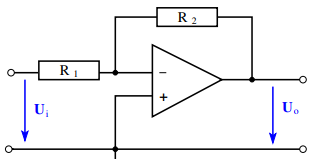
\includegraphics[width=0.5\textwidth]{invertierend.png}
    \caption{Schaltbild eines invertierenden Verstärkers \cite{ap51}.}
    \label{fig:verstaerker}
\end{figure}
\\
\textbf{Integrator}
Der Umkehrintegrator wird nach \autoref{fig:integrator} mit $R = 10\,\unit{\kilo\ohm}$ und 
$C = \,\text{nF}$ aufgebaut. Im Anschluss wird die Zeitkonstante überprüft. 
Es wird nun die Eingangs- und Ausgangsspannung in Abhängigkeit von der Frequenz gemessen. 
Dabei werden Eingangssignale in Form einer Dreicks- und Rechtecksspannung verwendet. Das Eingangssignal 
darf keine Gleichstromkomponenten enthalten.
\begin{figure}
    \centering
    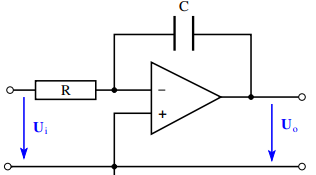
\includegraphics[width=0.5\textwidth]{integrator.png}
    \caption{Schaltbild eines Integrators \cite{ap51}.}
    \label{fig:integrator}
\end{figure}
\\
\textbf{Differenzierer}
Der Differenzierer wird mit $R=100\,\unit{\kilo\ohm}$ und $C=22\,\text{nF}$ wie in \autoref{fig:differenzierer}.
Auch hier wird die Eingangs- und Ausgangsspannung in Abhängigkeit von der Frequenz gemessen. Hierbei wir das Eingangssignal 
ebenfalls zwischen einer Dreieck- und Rechtecksspannung variiert.
\begin{figure}
    \centering
    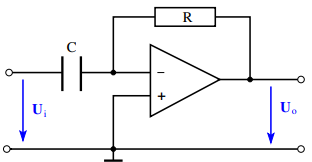
\includegraphics[width=0.5\textwidth]{differenzierer.png}
    \caption{Schaltbild eines Differenzierers \cite{ap51}.}
    \label{fig:differenzierer}
\end{figure}
\\
\textbf{Schmitt-Trigger}
Der Schmitt-Trigger wird nach \autoref{fig:schmitt} mit $R_1 = 10\,\unit{\kilo\ohm}$ und
$R_2=100\,\unit{\kilo\ohm}$ aufgebaut. Die Amplitude wird nun von $0\,\unit{\volt}$ an in $\unit{\milli\volt}$-Schritten 
erhöht. Mithilfe des Oszilloskops wird folglich der Hochpunkt gesucht. Dieser kann alternativ mittels einer 
Dreiecksspannung gefunden werden; dabei ist die Amplitude jedoch allgemein höher. Es werden mehrere Hochpunkte gesucht und im Anschluss gemittelt. 
Die Eingangs- und Ausgangsspannungen werden aufgrund der Hysterese zeitgleich notiert. 
\begin{figure}
    \centering
    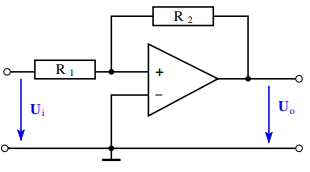
\includegraphics[width=0.5\textwidth]{schmitt.png}
    \caption{Schaltbild eines Schmitt-Triggers \cite{ap51}.}
    \label{fig:schmitt}
\end{figure}
\\
\textbf{Generator}
Für den Generator werden folgende Werte verwendet: $R_1= 10\,\unit{\kilo\ohm}$, $R_2=100\,\unit{\kilo\ohm}$,
$R_3=1\,\unit{\kilo\ohm}$ und $C=1\,\text{nF}$. Der Generator wird nach \autoref{fig:generator} aufgebaut. 
Das System startet spontan zu oszillieren und generiert eine Dreiecksspannung $U_a$.
\begin{figure}
    \centering
    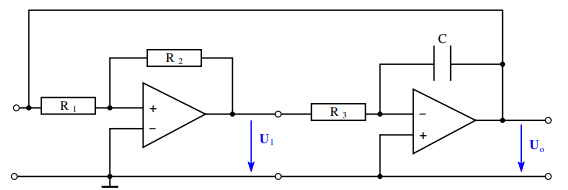
\includegraphics[width=0.7\textwidth]{generator.png}
    \caption{Schaltbild eines Generators \cite{ap51}.}
    \label{fig:generator}
\end{figure}
\\
\textbf{Generator mit variierenden Amplituden}
Der Generator mit variierenden Amplituden wird nach \autoref{fig:generatorvar} aufgebaut. Für die Kapazität kann $C=22\,\text{nF}$ oder 
$C=100\,\text{nF}$ gewählt werden. Es werden nun experimentell die Periode und die Umlaufdauer 
der Oszillation des Generators bestimmt. Dazu kann der Dämpfungsfaktor $\eta$ über das Potentiometer P zwischen -1 und 1 
eingestellt werden. Wenn der Dämpfungsfaktor negativ ist, zeichnet das Oszilloskop eine gedämpfte Oszillation auf. Hierbei muss das Eingangssignal 
eine Rechtecksschwingung sein, da das System nicht spontan zu oszillieren beginnt. Es wird die Dämpfung der Oszillation gemessen.
Wenn der Dämpfungsfaktor positiv ist, beginnt das System von allein zu oszillieren. Diesmal wird die Periode der Oszillation gemessen.  
\begin{figure}
    \centering
    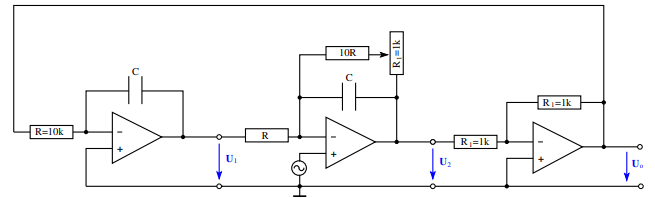
\includegraphics[width=0.8\textwidth]{generatorvar.png}
    \caption{Schaltbild eines Generators mit variierenden Amplituden \cite{ap51}.}
    \label{fig:generatorvar}
\end{figure}
\\